\documentclass[11pt,letterpaper]{article}
\usepackage[left=0.9in,right=0.9in,top=0.8in,bottom=0.85in]{geometry}
\usepackage[T1]{fontenc}
\usepackage{lmodern}
\usepackage{amsmath,amssymb,booktabs,array,tabularx}
\usepackage{xcolor}
\usepackage{tikz}
\usetikzlibrary{arrows.meta,positioning}
\usepackage[hidelinks]{hyperref}
\usepackage{xurl}
\usepackage{microtype}
\usepackage{caption}
\usepackage{titlesec}
\titleformat{\section}{\large\bfseries}{\thesection}{0.65em}{}
\titleformat{\subsection}{\normalsize\bfseries}{\thesubsection}{0.65em}{}
\titlespacing*{\section}{0pt}{2.2ex plus .5ex}{0.8ex}
\titlespacing*{\subsection}{0pt}{1.6ex plus .4ex}{0.6ex}
\titlespacing*{\paragraph}{0pt}{1.2ex plus .2ex}{0.7em}
\renewenvironment{abstract}{\par\medskip\noindent\textbf{Abstract}\par\smallskip\noindent\ignorespaces}{\par\medskip}
\setlength{\parindent}{0pt}
\setlength{\parskip}{5pt plus 1pt}
\captionsetup{font=small,labelfont=bf,skip=8pt}
\setlength{\textfloatsep}{12pt plus 3pt minus 2pt}
\setlength{\intextsep}{10pt plus 3pt minus 2pt}
\usepackage[section]{placeins}
\usepackage{float}
\widowpenalty=10000
\clubpenalty=10000
\raggedbottom
\definecolor{plotblue}{HTML}{3E7392}
\definecolor{plotgold}{HTML}{996510}
\definecolor{plotgreen}{HTML}{2F7D57}
\definecolor{plotgray}{HTML}{667085}
\definecolor{plotlight}{HTML}{E8F1F7}
\definecolor{plotpale}{HTML}{E7F4EC}
\tikzset{every picture/.style={font=\small},
 paperarrow/.style={-{Latex[length=2mm]},thick,draw=plotgray}}

\newcommand{\run}[1]{\texttt{#1}}
\newcommand{\draftnote}[1]{\par\smallskip{\footnotesize\color{plotgray}\noindent\textit{Draft note: #1}\par}\smallskip}
\setlength{\emergencystretch}{2em}
\title{TREC RAG 2026:\\Single-pass and Multi-stage Answer Generation}
\author{Nidhin Pattaniyil \and Tanwir Zaman \and Semih Yagli}
\date{}
\begin{document}
\begin{center}
{\Large\bfseries TREC RAG 2026\par}
\smallskip
{\large Single-pass and Multi-stage Answer Generation\par}
\medskip
\begin{tabular}{@{}c@{\hspace{1.5em}}c@{\hspace{1.5em}}c@{}}
Nidhin Pattaniyil & Tanwir Zaman & Semih Yagli\\[3pt]
{\footnotesize\href{mailto:npatta01@gmail.com}{\textcolor{plotblue}{npatta01@gmail.com}}} &
{\footnotesize\href{mailto:zaman.tanwir@gmail.com}{\textcolor{plotblue}{zaman.tanwir@gmail.com}}} &
{\footnotesize\href{mailto:semihyagli1@gmail.com}{\textcolor{plotblue}{semihyagli1@gmail.com}}}
\end{tabular}\\[5pt]
{\small Independent researchers $\cdot$ Team NP Labs}
\end{center}
\begin{abstract}
We compare two ways to answer TREC RAG requests using the same retrieved passages. Single-pass writes an answer directly. Multi-stage first plans an answer, then checks the draft for missing information and screens proposed edits. Multi-stage received higher organizer human-preference and coverage scores. On 25 topics, coverage of human-authored facts was 0.6578 versus 0.5705. We trace a submitted Green Bay topic from LLM-generated facets to evidence and both accepted answers. Three additional Retrieval baselines reuse the RAG pipeline's saved results.
\end{abstract}

\section{Start with the Questions Inside the Request}
TREC RAG supplies 119 long-form information requests, called \emph{narratives}. A system searches the ClimbMix document collection and writes an answer of at most 1,024 words, citing its sources~\cite{track2026}. \textbf{Input:} a request and access to the collection. \textbf{Output:} an answer with document citations.

A request often asks several things at once. We use DeepSeek V4 Flash to split it into \textbf{facets}: focused questions that each cover part of the request. The model also writes search queries for those questions. We also search the original request. Each topic can have up to eight facets with 1--3 queries each: at most 25 searches in total.

\begin{figure}[H]\centering
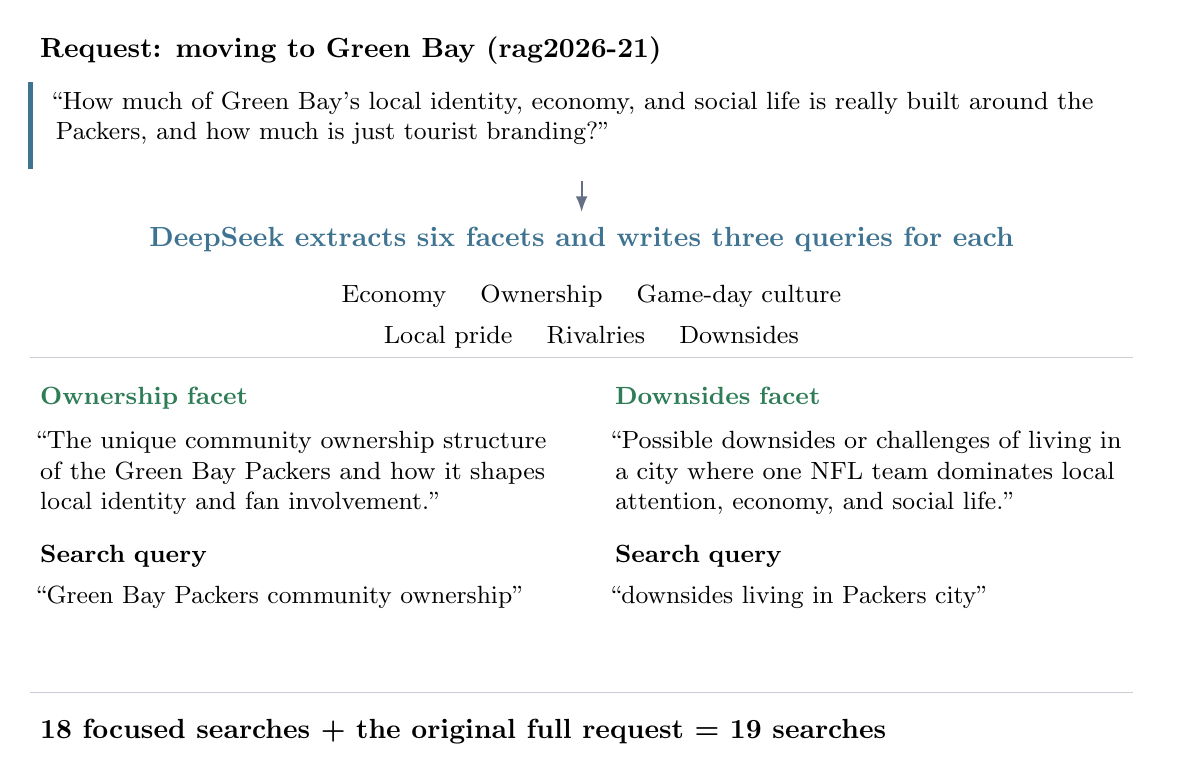
\begin{tikzpicture}[x=1cm,y=1cm,font=\small]
\node[anchor=west,font=\bfseries] at (0,0) {Request: moving to Green Bay (rag2026-21)};
\draw[plotblue,line width=2pt] (0,-.4)--(0,-1.5);
\node[anchor=north west,text width=13.5cm,align=left] at (.2,-.4)
 {``How much of Green Bay's local identity, economy, and social life is really built around the Packers, and how much is just tourist branding?''};
\draw[paperarrow] (7,-1.65)--(7,-2.05);
\node[font=\bfseries,text=plotblue] at (7,-2.4) {DeepSeek extracts six facets and writes three queries for each};
\node[anchor=north west,text width=14cm,align=center] at (0,-2.85)
 {Economy \quad Ownership \quad Game-day culture\\[4pt] Local pride \quad Rivalries \quad Downsides};
\draw[plotgray!35] (0,-3.9)--(14,-3.9);
\node[anchor=north west,text width=6.5cm,align=left] at (0,-4.15)
 {\textcolor{plotgreen}{\textbf{Ownership facet}}\\[5pt]
 ``The unique community ownership structure of the Green Bay Packers and how it shapes local identity and fan involvement.''\\[8pt]
 \textbf{Search query}\\[4pt]
 ``Green Bay Packers community ownership''};
\node[anchor=north west,text width=6.5cm,align=left] at (7.3,-4.15)
 {\textcolor{plotgreen}{\textbf{Downsides facet}}\\[5pt]
 ``Possible downsides or challenges of living in a city where one NFL team dominates local attention, economy, and social life.''\\[8pt]
 \textbf{Search query}\\[4pt]
 ``downsides living in Packers city''};
\draw[plotgray!35] (0,-8.15)--(14,-8.15);
\node[anchor=west,font=\bfseries] at (0,-8.65) {18 focused searches + the original full request = 19 searches};
\end{tikzpicture}
\caption{DeepSeek splits the Green Bay request into six facets. Two facets and their search queries are shown below the full set of headings.}
\label{fig:facets}
\end{figure}

\clearpage
\section{Turn Retrieved Documents into Evidence and Nuggets}
We create the passages ourselves from retrieved ClimbMix documents. Before either writer runs, we select exact source text and use Nuggetizer~\cite{nuggetizer2025} to turn it into short, evidence-linked claims. These generated nuggets are advisory hints, not organizer gold nuggets.

\begin{figure}[H]\centering
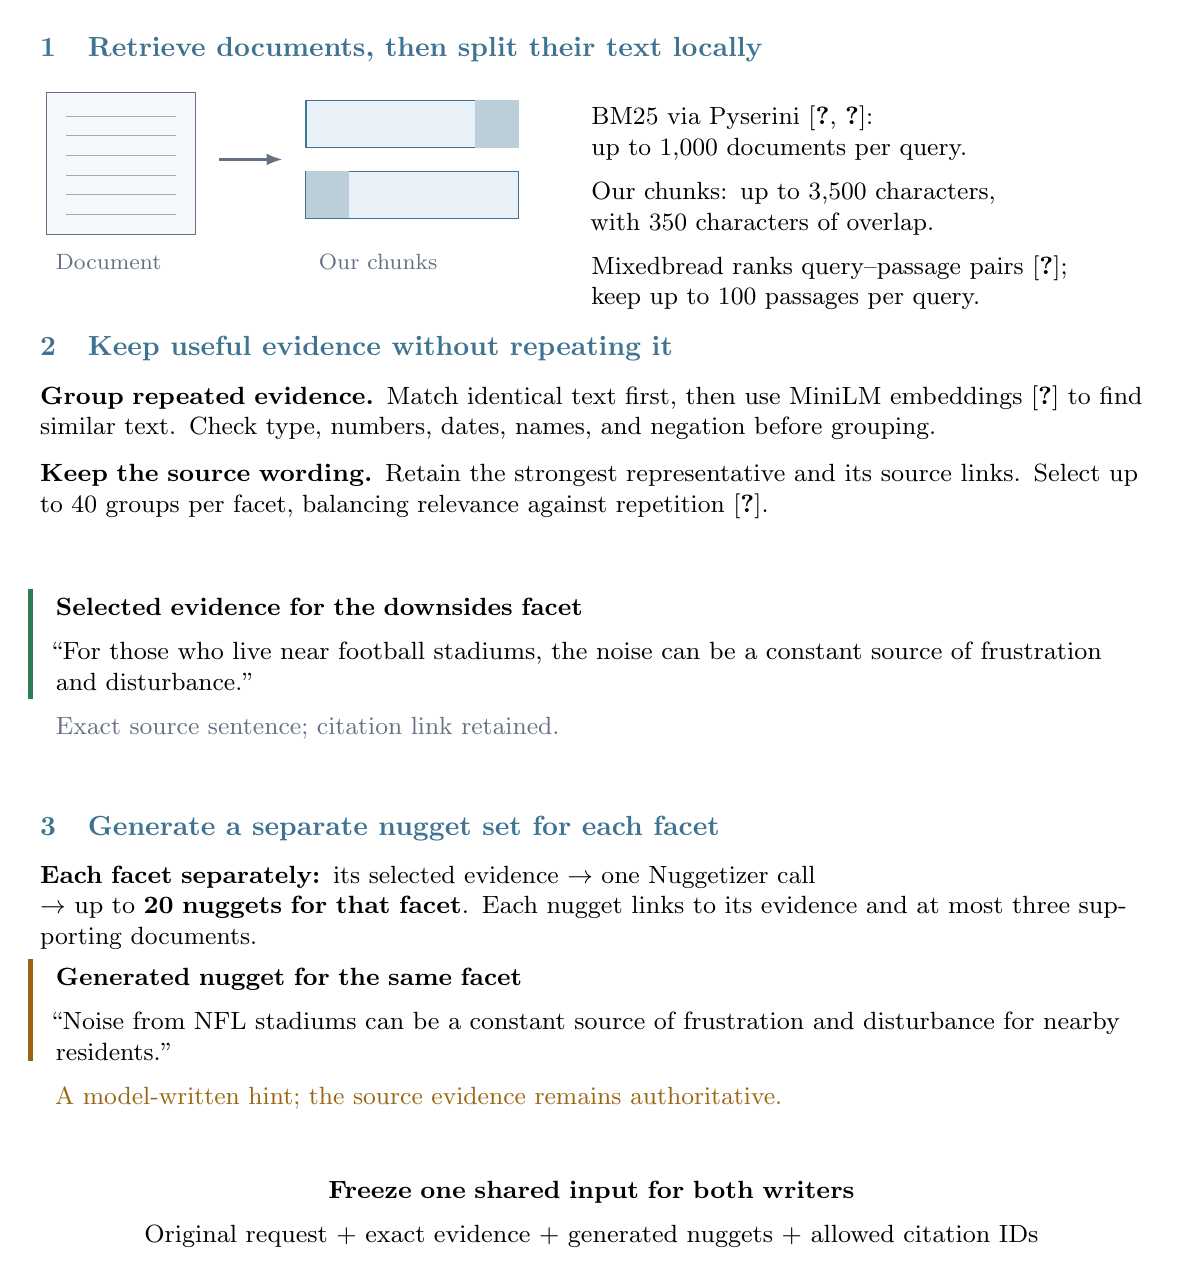
\begin{tikzpicture}[x=1cm,y=1cm,font=\small]
\node[anchor=west,font=\bfseries,text=plotblue] at (0,0) {1\quad Retrieve documents, then split their text locally};
% Document and overlapping passage strips show the unit change.
\draw[plotgray,fill=plotlight!40] (.2,-0.55) rectangle (2.1,-2.35);
\foreach \y in {-.85,-1.1,-1.35,-1.6,-1.85,-2.1}
 {\draw[plotgray!60] (.45,\y)--(1.85,\y);}
\draw[paperarrow] (2.4,-1.4)--(3.2,-1.4);
\draw[plotblue,fill=plotlight] (3.5,-0.65) rectangle (6.2,-1.25);
\draw[plotblue,fill=plotlight] (3.5,-1.55) rectangle (6.2,-2.15);
\fill[plotblue!35] (5.65,-1.25) rectangle (6.2,-0.65);
\fill[plotblue!35] (3.5,-2.15) rectangle (4.05,-1.55);
\node[anchor=north west,text width=6.8cm,align=left] at (7,-0.6)
 {BM25 via Pyserini~\cite{bm25,pyserini}:\\up to 1,000 documents per query.\\[5pt]
 Our chunks: up to 3,500 characters,\\with 350 characters of overlap.\\[5pt]
 Mixedbread ranks query--passage pairs~\cite{mixedbread};\\keep up to 100 passages per query.};
\node[anchor=west,font=\footnotesize,text=plotgray] at (.2,-2.7)
 {Document \hspace{1.8cm} Our chunks};

\node[anchor=west,font=\bfseries,text=plotblue] at (0,-3.8) {2\quad Keep useful evidence without repeating it};
\node[anchor=north west,text width=14cm,align=left] at (0,-4.15)
 {\textbf{Group repeated evidence.} Match identical text first, then use MiniLM embeddings~\cite{minilm} to find similar text. Check type, numbers, dates, names, and negation before grouping.\\[6pt]
 \textbf{Keep the source wording.} Retain the strongest representative and its source links. Select up to 40 groups per facet, balancing relevance against repetition~\cite{mmr}.};
\draw[plotgreen,line width=2pt] (0,-6.85)--(0,-8.25);
\node[anchor=north west,text width=13.5cm,align=left] at (.2,-6.85)
 {\textbf{Selected evidence for the downsides facet}\\[5pt]
 ``For those who live near football stadiums, the noise can be a constant source of frustration and disturbance.''\\[5pt]
 \textcolor{plotgray}{Exact source sentence; citation link retained.}};

\node[anchor=west,font=\bfseries,text=plotblue] at (0,-9.9) {3\quad Generate a separate nugget set for each facet};
\node[anchor=north west,text width=14cm,align=left] at (0,-10.25)
 {\textbf{Each facet separately:} its selected evidence $\rightarrow$ one Nuggetizer call\\$\rightarrow$ up to \textbf{20 nuggets for that facet}. Each nugget links to its evidence and at most three supporting documents.};
\draw[plotgold,line width=2pt] (0,-11.55)--(0,-12.85);
\node[anchor=north west,text width=13.5cm,align=left] at (.2,-11.55)
 {\textbf{Generated nugget for the same facet}\\[5pt]
 ``Noise from NFL stadiums can be a constant source of frustration and disturbance for nearby residents.''\\[5pt]
 \textcolor{plotgold}{A model-written hint; the source evidence remains authoritative.}};

\node[anchor=north west,text width=14cm,align=center] at (0,-14.25)
 {\textbf{Freeze one shared input for both writers}\\[5pt]
 Original request + exact evidence + generated nuggets + allowed citation IDs};
\end{tikzpicture}
\caption{From retrieved documents to shared writer input: split the text, select evidence, then generate nuggets for each facet. The Green Bay example shows a source sentence and its linked nugget.}
\label{fig:evidence-preparation}
\end{figure}

Nuggets help organize the answer; writers must ground their claims in the original evidence. Both writers receive the same request, evidence, and nuggets. Neither searches again or reads organizer judgments. This decomposition-and-selection approach builds on earlier TREC systems~\cite{tus2025,wing2025}.

\clearpage
\section{Write Two Answers from the Same Evidence}
GPT-5.6 Sol writes both answers. Single-pass writes directly from the shared evidence. Multi-stage adds GPT-5.6 Luna to plan the answer, look for omissions, and screen proposed edits.

\begin{figure}[H]\centering
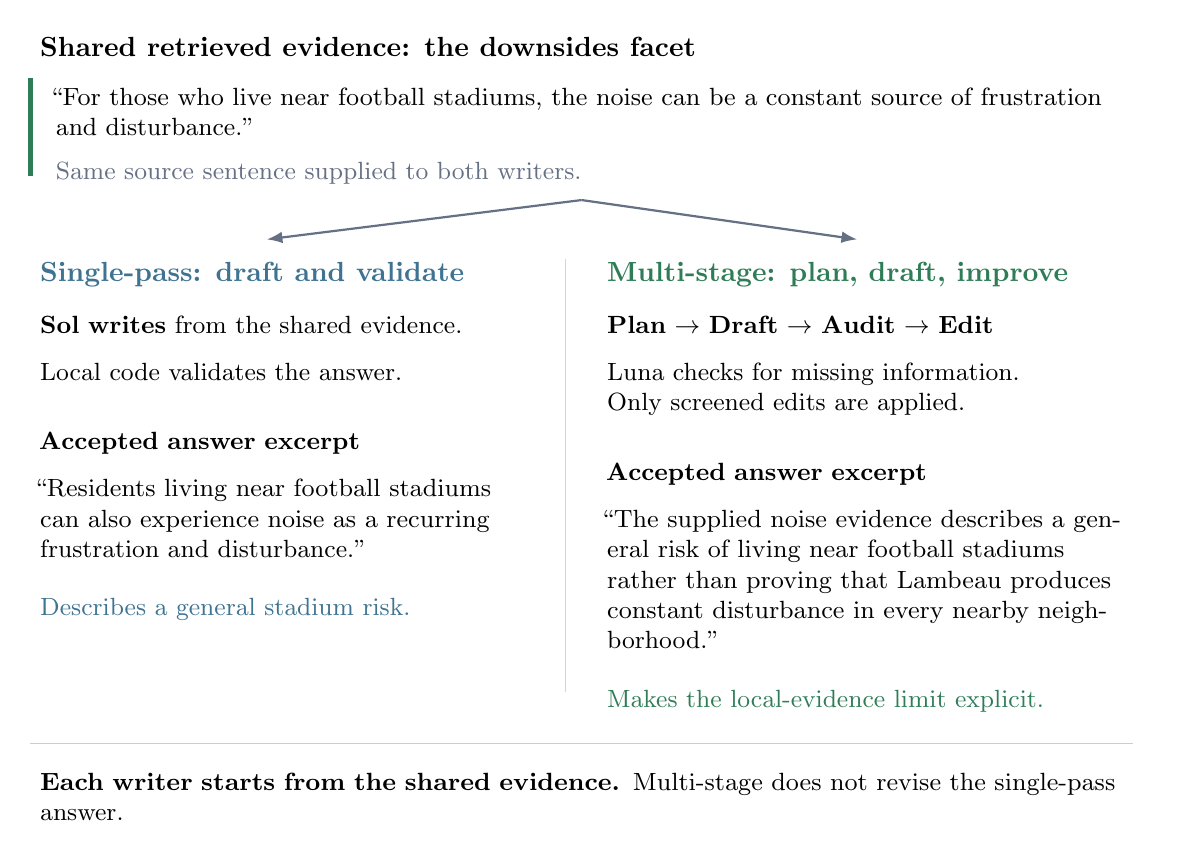
\begin{tikzpicture}[x=1cm,y=1cm,font=\small]
\node[anchor=west,font=\bfseries] at (0,0) {Shared retrieved evidence: the downsides facet};
\draw[plotgreen,line width=2pt] (0,-.4)--(0,-1.65);
\node[anchor=north west,text width=13.4cm,align=left] at (.2,-.4)
 {``For those who live near football stadiums, the noise can be a constant source of frustration and disturbance.''\\[5pt]
 \textcolor{plotgray}{Same source sentence supplied to both writers.}};
\draw[paperarrow] (7,-1.95)--(3,-2.45);
\draw[paperarrow] (7,-1.95)--(10.5,-2.45);
\node[anchor=west,font=\bfseries,text=plotblue] at (0,-2.9) {Single-pass: draft and validate};
\node[anchor=west,font=\bfseries,text=plotgreen] at (7.2,-2.9) {Multi-stage: plan, draft, improve};
\draw[plotgray!30] (6.8,-2.7)--(6.8,-8.2);
\node[anchor=north west,text width=6.2cm,align=left] at (0,-3.3)
 {\textbf{Sol writes} from the shared evidence.\\[6pt]
 Local code validates the answer.\\[14pt]
 \textbf{Accepted answer excerpt}\\[6pt]
 ``Residents living near football stadiums can also experience noise as a recurring frustration and disturbance.''\\[10pt]
 \textcolor{plotblue}{Describes a general stadium risk.}};
\node[anchor=north west,text width=6.6cm,align=left] at (7.2,-3.3)
 {\textbf{Plan $\rightarrow$ Draft $\rightarrow$ Audit $\rightarrow$ Edit}\\[6pt]
 Luna checks for missing information.\\Only screened edits are applied.\\[14pt]
 \textbf{Accepted answer excerpt}\\[6pt]
 ``The supplied noise evidence describes a general risk of living near football stadiums rather than proving that Lambeau produces constant disturbance in every nearby neighborhood.''\\[10pt]
 \textcolor{plotgreen}{Makes the local-evidence limit explicit.}};
\draw[plotgray!35] (0,-8.85)--(14,-8.85);
\node[anchor=north west,text width=14cm,align=left] at (0,-9.1)
 {\textbf{Each writer starts from the shared evidence.} Multi-stage does not revise the single-pass answer.};
\end{tikzpicture}
\caption{Answer excerpts for the Green Bay topic. Both cite the same source; multi-stage explicitly distinguishes a general stadium risk from evidence about Lambeau.}
\label{fig:revision}
\end{figure}

Sol proposes edits; Luna screens them for support, usefulness, repetition, and lost qualifications. Local code applies accepted edits and checks citations and length. Multi-stage keeps the validated draft if revision fails. Both methods produced 119 answers that passed these format checks.

\clearpage
\section{Organizer RAG Results}
Multi-stage scored higher on both human preference and information coverage. The organizer evaluated subsets of the 119 submitted topics~\cite{organizer2026}. Reference medians weight runs equally, rather than teams; they do not give our leaderboard rank.

\paragraph{Human preference.}
Human assessors compared answers in two disjoint batches: 17 topics with narrative-based rubrics, and 25 topics with expected facts gathered from the corpus. The organizer fitted Bradley--Terry preference ratings separately for each batch. Multi-stage was above the run median in both; single-pass was below it in Batch 1 and near it in Batch 2.

\begin{table}[H]\centering\small
\begin{tabular}{@{}lrrr@{}}\toprule
Batch & Single-pass [95\% CI] & Multi-stage [95\% CI] & Run median\\\midrule
1 (17 topics) & 1019.7 [970.5, 1068.9] & 1179.8 [1128.6, 1231.0] & 1048.7\\
2 (25 topics) & 1026.0 [983.8, 1068.3] & 1181.4 [1134.6, 1228.2] & 1024.8\\\bottomrule
\end{tabular}
\caption{Organizer human-preference ratings. Higher is better. Each batch has its own fitted Bradley--Terry scale; compare systems within a row.}
\label{tab:official-preference}
\end{table}

The 95\% intervals do not overlap within either batch. They use a judgment-level sandwich estimator; we performed no additional paired significance test.

\paragraph{Information coverage.}
Coverage was judged by GPT-6.1 Sol at medium reasoning. \emph{Vital strict} counts the proportion of essential items fully supported by an answer; \emph{all strict} includes all items equally. Partial support earns no credit. The three collections are reported separately in Table~\ref{tab:official-coverage}.

\begin{table}[H]
\centering\small
\begin{tabular}{@{}llrrr@{}}
\toprule
Collection & Measure & Single-pass & Multi-stage & Run median\\
\midrule
Batch 1 rubrics (17) & Vital strict & 0.8431 & 0.8804 & 0.7157\\
 & All strict & 0.7740 & 0.8738 & 0.7325\\
\midrule
Batch 2 human nuggets (25) & Vital strict & 0.5383 & 0.6338 & 0.4879\\
 & All strict & 0.5705 & 0.6578 & 0.5556\\
\midrule
Batch 2 automatic nuggets (25) & Vital strict & 0.1647 & 0.3147 & 0.1547\\
 & All strict & 0.1280 & 0.2496 & 0.1280\\
\bottomrule
\end{tabular}
\caption{Organizer RAG coverage scores, averaged equally across topics within each collection. Higher is better. Medians summarize evaluated runs, not teams. The collections contain different items and should not be compared as if they were one test.}
\label{tab:official-coverage}
\end{table}

Multi-stage scored higher on all six coverage measures. On human-authored Batch-2 nuggets, the gain over single-pass was 8.73 percentage points (0.6578 versus 0.5705). Both exceeded the run median for that measure.



\clearpage
\section{Derived Retrieval Baselines}
\label{sec:retrieval}
The Retrieval task asks for a ranked document list. Our three baselines reuse the RAG pipeline's saved searches and passage scores. Within each narrative or facet pool, we keep documents whose scores stand well above the typical score, using a cutoff adjusted for the spread of scores. We combine these selections into one document set. Each run contains the same 4,246 topic--document pairs, returning 1--121 documents per topic.

\begin{figure}[H]\centering
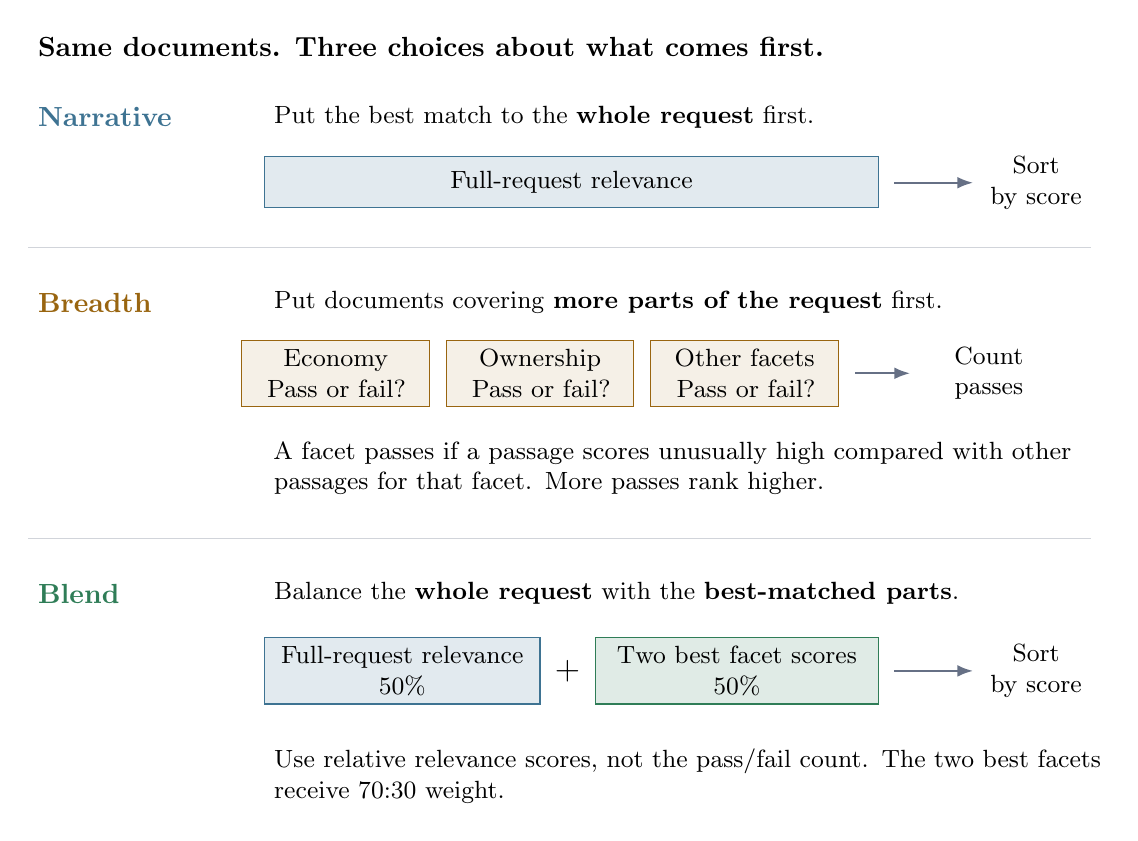
\begin{tikzpicture}[x=1cm,y=1cm,font=\small]
\node[anchor=west,font=\bfseries] at (0,0) {Same documents. Three choices about what comes first.};
\node[anchor=west,font=\bfseries,text=plotblue] at (0,-.9) {Narrative};
\node[anchor=west] at (3,-.9) {Put the best match to the \textbf{whole request} first.};
\draw[fill=plotblue!15,draw=plotblue] (3,-1.4) rectangle (10.8,-2.05);
\node at (6.9,-1.73) {Full-request relevance};
\draw[paperarrow] (11,-1.73)--(12,-1.73);
\node[align=center] at (12.8,-1.73) {Sort\\by score};
\draw[plotgray!30] (0,-2.55)--(13.5,-2.55);
\node[anchor=west,font=\bfseries,text=plotgold] at (0,-3.25) {Breadth};
\node[anchor=west] at (3,-3.25) {Put documents covering \textbf{more parts of the request} first.};
\foreach \x/\facetname in {3.9/Economy,6.5/Ownership,9.1/Other facets} {
 \node[draw=plotgold,fill=plotgold!10,text width=2.15cm,minimum height=.75cm,align=center] at (\x,-4.15) {\facetname\\Pass or fail?};}
\draw[paperarrow] (10.5,-4.15)--(11.2,-4.15);
\node[align=center] at (12.2,-4.15) {Count\\passes};
\node[anchor=north west,text width=10.5cm,align=left] at (3,-4.9)
 {A facet passes if a passage scores unusually high compared with other passages for that facet. More passes rank higher.};
\draw[plotgray!30] (0,-6.25)--(13.5,-6.25);
\node[anchor=west,font=\bfseries,text=plotgreen] at (0,-6.95) {Blend};
\node[anchor=west] at (3,-6.95) {Balance the \textbf{whole request} with the \textbf{best-matched parts}.};
\draw[fill=plotblue!15,draw=plotblue] (3,-7.5) rectangle (6.5,-8.35);
\node[align=center] at (4.75,-7.93) {Full-request relevance\\50\%};
\node[font=\large] at (6.85,-7.93) {+};
\draw[fill=plotgreen!15,draw=plotgreen] (7.2,-7.5) rectangle (10.8,-8.35);
\node[align=center] at (9,-7.93) {Two best facet scores\\50\%};
\draw[paperarrow] (11,-7.93)--(12,-7.93);
\node[align=center] at (12.8,-7.93) {Sort\\by score};
\node[anchor=north west,text width=10.5cm,align=left] at (3,-8.8)
 {Use relative relevance scores, not the pass/fail count. The two best facets receive 70:30 weight.};
\end{tikzpicture}
\caption{The three derived Retrieval baselines change the ordering, not the document set. Narrative and Blend use percentile relevance scores. Breadth counts facets passing a raw-score threshold, breaking ties by strong-passage count and then Blend.}
\label{fig:retrieval-orderings}
\end{figure}

On 82 topics, automated UMBRELA judgments~\cite{umbrela} treated relevance grades of at least 2 as relevant. Precision measures the relevant share of returned documents; recall measures the share of judged-relevant documents returned. We had higher precision but lower recall than the run median (Table~\ref{tab:official-retrieval}).

\begin{table}[H]
\centering\small
\begin{tabular}{@{}lrrr@{}}
\toprule
Measure & Topics & All three runs & Run median\\
\midrule
Document precision & 82 & 0.4116 & 0.3499\\
Document recall & 82 & 0.0897 & 0.1002\\
Mean submitted documents & 82 & 38.6 & 100.0\\
\midrule
Gain: human-authored nuggets & 25 & 0.7839 & 0.8965\\
Gain: automatic nuggets & 25 & 0.4033 & 0.6268\\
Mean submitted documents & 25 & 31.8 & 100.0\\
\bottomrule
\end{tabular}
\caption{Organizer Retrieval results. Medians cover 114 evaluated runs from 27 teams, weighting each run equally. Scores and document counts are topic means; the two count rows use different topic subsets. Higher precision, recall, and gain are better; document count describes effort.}
\label{tab:official-retrieval}
\end{table}

On 25 topics, the organizer also measured coverage of expected facts, or nuggets. Each fully supported nugget counts once, weighted 1 for essential facts and 0.5 for other useful facts. Assignments were automated for both human-authored and automatic nuggets. Both gain scores were below the run medians.

All three rankings received identical scores, including per-topic scores: the evaluation measures the full document set, which the rankings share. These results assess our selection, not which ordering puts useful documents first.



\section{What the RAG Comparison Establishes}
With the same evidence, multi-stage received higher human-preference and coverage scores. It also wrote longer answers: 531--1,011 words versus 203--749. Planning, auditing, revision, model mix, and length all changed together. We cannot attribute the improvement to one stage.

A separate retrospective citation-support check favored single-pass; the organizer gains should not be read as better citation grounding.

The organizer results favor the complete multi-stage configuration under fixed evidence. They do not isolate which stage caused the gain or whether answer length explains it. Retrieval coverage and citation support remain separate evaluation dimensions.

{\small\paragraph{Implementation and assistance.} The RAG runs were \run{rag26-ss1} (Single-pass) and \run{rag26-ms1-final} (Multi-stage, priority 1). Blend (\run{r26-narr-facet-v1}) was the prioritized Retrieval baseline. Accepted files remain unchanged. Codex assisted development, analysis, and drafting; author review is pending.}

\begingroup\small
\begin{thebibliography}{99}
\bibitem{organizer2026}
TREC RAG Track Organizers. \emph{Retrieval and RAG task results}. Participant-specific TSV score releases and accompanying evaluation READMEs, received November 2026; inspected November 7, 2026. Includes overall run reference statistics. Unpublished participant communication.

\bibitem{track2026}
TREC RAG organizers. \emph{TREC RAG 2026: Retrieval-Augmented Generation Track}. 2026. \url{https://trec-rag.github.io/}. Accessed November 7, 2026.
\bibitem{nuggetizer2025}
Ronak Pradeep, Nandan Thakur, Shivani Upadhyay, Daniel Campos, Nick Craswell, and Jimmy Lin. \emph{The Great Nugget Recall: Automating Fact Extraction and RAG Evaluation with Large Language Models}. In Proceedings of the 48th International ACM SIGIR Conference on Research and Development in Information Retrieval, pages 180--190, 2025. Software: \url{https://github.com/castorini/nuggetizer}.

\bibitem{tus2025}
Yukio Uematsu, Koyuki Otani, Tomoyuki Shiroyama, and Masaaki Tsuchida. \emph{Keystone-Docs RAG at TREC 2025: Coverage-Aware Few-Document Augmentation via Narrative Decomposition}. In Proceedings of TREC 2025. \url{https://trec.nist.gov/pubs/trec34/papers/tus.rag.pdf}.
\bibitem{wing2025}
Zizhen Li and Hai-Tao Yu. \emph{Submodular Evidence Selection for Grounded Answer Generation in TREC RAG 2025}. In Proceedings of TREC 2025. \url{https://trec.nist.gov/pubs/trec34/papers/WING-II.rag.pdf}.

\bibitem{bm25}
Stephen Robertson and Hugo Zaragoza. \emph{The Probabilistic Relevance Framework: BM25 and Beyond}. Foundations and Trends in Information Retrieval, 3(4):333--389, 2009. \url{https://doi.org/10.1561/1500000019}.

\bibitem{pyserini}
Jimmy Lin, Xueguang Ma, Sheng-Chieh Lin, Jheng-Hong Yang, Ronak Pradeep, and Rodrigo Nogueira. \emph{Pyserini: A Python Toolkit for Reproducible Information Retrieval Research with Sparse and Dense Representations}. SIGIR, pages 2356--2362, 2021. \url{https://github.com/castorini/pyserini}.

\bibitem{mixedbread}
Xianming Li, Aamir Shakir, Rui Huang, Julius Lipp, Benjamin Clavi\'e, and Jing Li. \emph{ProRank: Prompt Warmup via Reinforcement Learning for Small Language Models Reranking}. arXiv:2506.03487, 2025. Model used: \texttt{mxbai-rerank-base-v2}. \url{https://arxiv.org/abs/2506.03487}.

\bibitem{minilm}
Sentence Transformers. \emph{all-MiniLM-L6-v2}. Model card. \url{https://huggingface.co/sentence-transformers/all-MiniLM-L6-v2}. Accessed November 7, 2026.

\bibitem{mmr}
Jaime Carbonell and Jade Goldstein. \emph{The Use of MMR, Diversity-Based Reranking for Reordering Documents and Producing Summaries}. SIGIR, pages 335--336, 1998. \url{https://doi.org/10.1145/290941.291025}.

\bibitem{umbrela}
Shivani Upadhyay, Ronak Pradeep, Nandan Thakur, Nick Craswell, and Jimmy Lin. \emph{UMBRELA: UMbrela is the (Open-Source Reproduction of the) Bing RELevance Assessor}. arXiv:2406.06519, 2024. \url{https://arxiv.org/abs/2406.06519}.

\end{thebibliography}
\endgroup
\end{document}
